\documentclass[./../../paper.tex]{subfiles}
\graphicspath{{\subfix{./../../figures/}}}

\begin{document}

\section{Determine the best Number of Cycles for the Evolutionary Algorithm }

\subsection{Experimental Setup}
\label{sec:exp3}
Given the chosen configuration from \autoref{sec:exp1} and the chosen hyperparameters of \autoref{sec:exp2}, we explore the effects of different stopping criterions for the evolutionary algorithm. The goal is to find a stopping criterion which yields reasonably good counterfactuals, while reducing the computation time. We will only consider the number of iterative cycles as a stopping criterion. We refer to each different criterion as termination point. Hence, a termination point at 5 means the algorithm, will not proceeed to optimize its results, further after reaching the fifth iteration.

We choose to run the configuration for evolution cycles from 5 to 100 in steps of 5. We keep the mutation rate at \attention{0.1} for each mutation type. The remaining procedure follows the process described in \autoref{sec:exp1}.

\subsection{Results}
\begin{figure}[htbp]
    \centering
    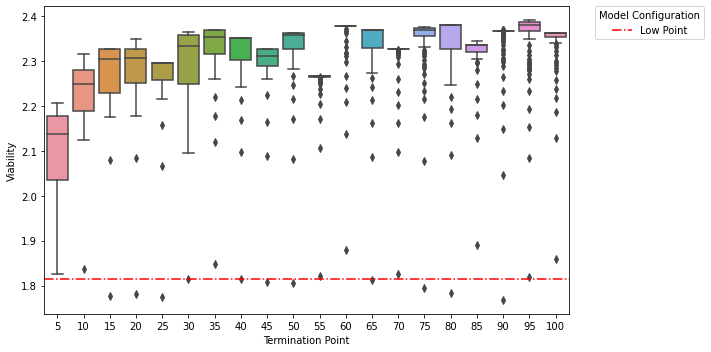
\includegraphics[width=\textwidth]{figures/generated/exp3_cycles_spread.png}
    \caption{This figure shows boxplots for the viability of each maximum number of iteration cycles tested. The x-axis shows how the viability evolves for each termination point.}
    \label{fig:exp3-normalized-lineplot}
\end{figure}

In \autoref{fig:exp3-normalized-lineplot}, we see a general increase in viability for each termination point. It shows, that increasing the termination point also yields better results at the end of the episode\attention{introduce term 'episode'}. However, the results do converge towards a viability of \attention{2.5}. Hence, increasing the termination point further is unlikely to generate better results.  

\begin{figure}[htbp]
    \centering
    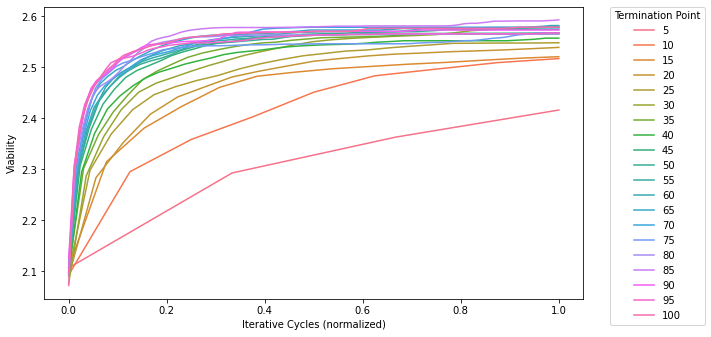
\includegraphics[width=\textwidth]{figures/generated/exp3_relative_cycles.png}
    \caption{shows the viability reached given the termination point. All termination points are normalized for better comparability.}
    \label{fig:exp3-iterations-boxplots}
\end{figure}


Furthermore, in \autoref{fig:exp3-iterations-boxplots} reflects the spread of the indivual results. Unsurprisingly, low termination points yields a larger spread dispersion of viability. The values become less dispersed, the higher the termination point. \optional{However, there are some surprising outliers. First, the termination points 55, 60 and 90 seem to have an extremely low dispersion. Meaning most of their results have the same viability. It is not clear whether this is a rule or mere coincindence.} Also, the number of outliers increase with the termination point as well. A last noteworthy observation is the amount of solutions near the mark of \attention{1.8}, as depicted with the dotted line.

\subsection{Discussion}
Most of the result were expected. The longer the algorithm runs, the more it narrows its solution space. Typically, this is a favorable characteristic. However, for counterfactual explanations, this advatange becomes a nuisance. We generally seek more diverse solutions. As discussed in \autoref{sec:viability}, we favor diverse solutions, but this aspect is not reflected in the viability measure. 

The low dispersion cases are probably solutions that are stuck in local optima. As mentioned earlier, this is a common flaw for evolutionary algorithms.

With regards to the low viability outliers, we can safely ignore those as we are mostly interested in the higher ranking counterfactuals.

% TODO: Need to align the distinction between viability measure and viability components. 
% TODO: Need to align naming of delta towards somethin better. Maybe Classification measure.

For the next experiments we are going to use \attention{35} as a termination point. This number is high enough to yield reasonable counterfactuals with high viability, while not being to narrow in its soltuin space.
\end{document}